\chapter{Viewing library} %{{{
\label{cha:Viewing library}

This chapter will present some visualization library which could be use to generate and interract with the component diagram. The comparison between those library is based on the features we want to offer to the KlugHDL user (see chapter \ref{sec:Goal}). In order to compare those viewing library, we end by discuting the point of the evaluation and the evaluation of all the library mentinnoed.

For the presentation of each of those library for graph visualization, we would use the same graph showed in figure \ref{fig:graph-base-model}.

\begin{figure}[h] % {{{ figure
    \centering
    \fbox{
        \digraph[scale=0.5]{GraphBaseModel}{
            node [shape=record];
            graph [rankdir=LR, 
                   ranksep="1", 
                   nodesep="1"];
            AndGate [label="{{<a>io.a : Bool|<b>io.b : Bool}|AndGate|{<c>io.c : Bool}}"];
            OrGate [label="{{<a>io.a : Bool|<b>io.b : Bool}|OrGate|{<c>io.c : Bool}}"];
            Input [label="{Input|{<a>io.a : Bool|<b>io.b : Bool}}"];
            Output [label="{{<c>io.c : Bool}|Output}"];
            Input:a -> AndGate:a;
            Input:b -> AndGate:b;
            Input:a -> OrGate:a;
            Input:b -> OrGate:b;
            OrGate:c -> Output:c;
            AndGate:c -> Output:c;
        }
    }
    \caption[Graph model for the viewing library comparison]
    {The graph model we will use for the incoming comparison
    between several Viewing library. This model includes two logical component : a AND and a OR gate and two nodes
    which are representing the input and output of the parent component}
    \label{fig:graph-base-model}
\end{figure} % }}}

\section{GraphStream} %{{{
\label{sec:Graphstream}

GraphStream is a Java library for the modeling and analysis of dynamic graphs\cite{graphstream}. The goal of the library is to provide a way to represents graphs and work on it\cite{graphstream}. GraphStream is an active project hosted by the university of Le Havre in France.

\subsection{Implementation} %{{{
\label{sub:Implementation}

The figure \ref{fig:base-graph-model-graphstream} show the base graph model realized with the GraphStream library.

\begin{figure}[h]
    \centering
    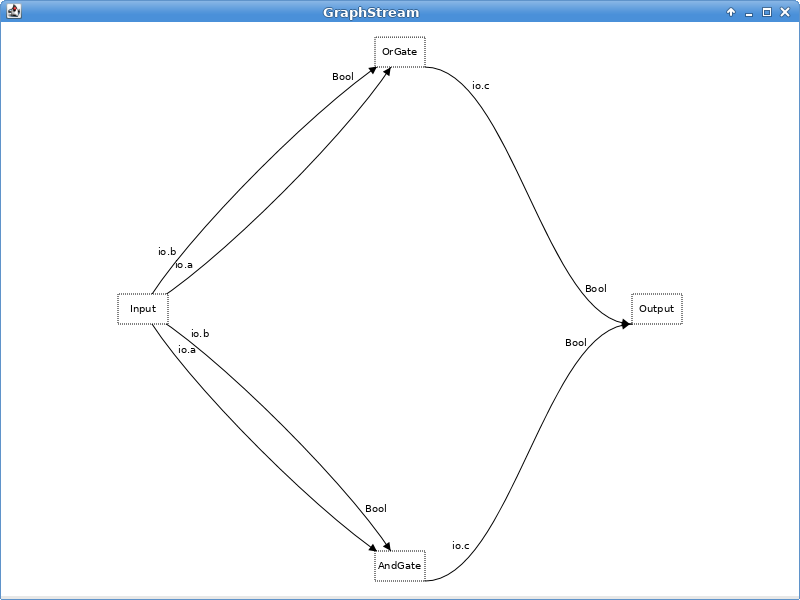
\includegraphics[width=0.8\textwidth]{img/graphstream-base-model-example}
    \caption{The base graph model rendering using graphstream}
    \label{fig:base-graph-model-graphstream}
\end{figure}

TODO : code example of Graphstream

%}}} subsection Implementation

\subsection{Remarks} %{{{
\label{sub:Remarks}

With GraphStream, there is no way to control some visual features which are very interresing for hardware component visualisation : the splines of the edges and the anchor position on the node. There is no way to have a node with sub-node like in the base graph model in figure \ref{fig:graph-base-model}.

An another special case is the label on the edges. With GraphStream, we could add some label on the edges like in listings \ref{lst:graphstream-edge-label}, but we can't add multiple ones. To add multiple label we need to use sprite like in listing \ref{lst:graphstream-edge-sprite}.

\begin{listing}[h] % {{{
    \centering
    \javafile{../ViewingLibrary/GraphstreamTest/src/examples/EdgesLabel.java}
    \caption{Add a label on an edge with GraphStream}
    \label{lst:graphstream-edge-label}
\end{listing} %}}}

\begin{listing}[h] % {{{
    \centering
    \javafile{../ViewingLibrary/GraphstreamTest/src/examples/SpriteEdgesExample.java}
    \caption{Add two label on an edge with GraphStream}
    \label{lst:graphstream-edge-sprite}
\end{listing} %}}}

%}}} subsection Remarks

GraphStream ownes some another features which could be usefull to design an application :
\begin{itemize}
    \item View integration using Swing
    \item Human-Computer interaction with the view
    \item A complete CSS interpretation to personalize the nodes and the edges
\end{itemize}

The main problem using GraphStream is we need to indicates the component information using label on the edges. The figure \ref{fig:base-graph-model-graphstream} show four nodes and six connections, but
if we have a more lot of edges between nodes, it would be difficult to see the types, like show in figure \ref{fig:graphstream-lot-of-edges}.

\begin{figure}
    \centering
    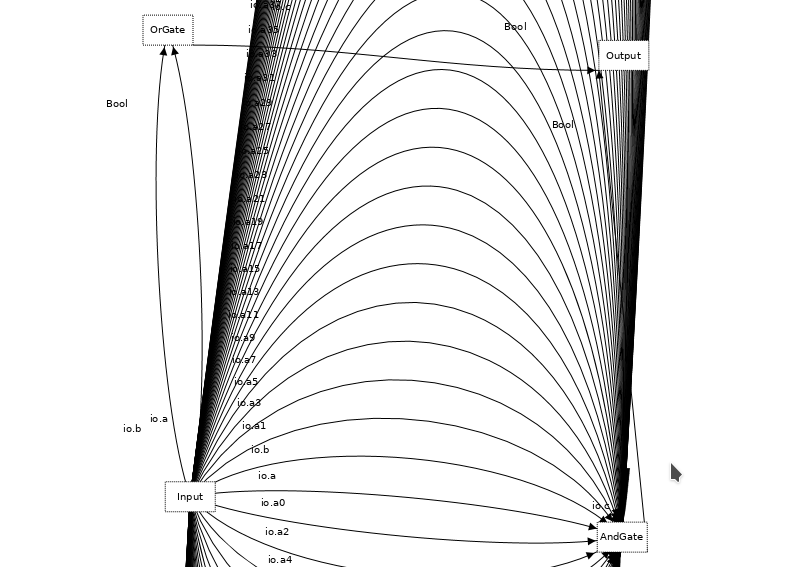
\includegraphics[width=0.8\textwidth]{img/graphstream_lot_of_edges}
    \caption[Label on multiple edges using Graphstream]{}
    \label{fig:graphstream-lot-of-edges}
\end{figure}


%}}} section Graphstream

\section{Draw2D} %{{{
\label{sec:Draw2D}

TODO

\subsection{Drage}

%}}} section Draw2D

%}}} chapter Viewing library 

